\documentclass[11pt]{article}
\usepackage[english]{babel}
\usepackage{url}
\usepackage{graphicx,DCCN2020_en}

\pagestyle{fancy}
\fancyhead{} 
\fancyfoot{}

\usepackage[utf8]{inputenc}
\linespread{1.0}

\usepackage{amsmath}

\makeatletter
\fancyhead[RO]{\small DCCN 2020\\ {14-18 September 2020}}
\fancyhead[LO]{\small P.D. Petrov, G.B. Kostadinov, et al. \\ Approximate Sequencing of Virtual Reels with GA}

\c@page=1
       
\makeatother

\title{Approximate Sequencing of Virtual Reels with Genetic Algorithms}

\author[]{\small P.D. Petrov}
\author[]{\small G.B. Kostadinov}
\author[]{\small P.R. Zhivkov}
\author[]{\small \\V.I. Velichkova}
\author[]{\small T.D. Balabanov\textsuperscript{0000-0003-3139-069X}}
\affil[]{\footnotesize Bulgarian Academy of Sciences \\ Institute of Information and Communication Technologies \\ acad. Georgi Bonchev Str., block 2, office 514 \\ 1113 Sofia, Bulgaria \\ http://iict.bas.bg/}
\email{p.petrov@iit.bas.bg g.kostadinov@iit.bas.bg pzhivkov@iit.bas.bg vvelichkova@iit.bas.bg todorb@iinf.bas.bg}
%
% Plamen Dimitrov Petrov - p.petrov@iit.bas.bg
% Georgi Borisov Kostadinov - g.kostadinov@iit.bas.bg
% Petar Rumenov Zhivkov - pzhivkov@iit.bas.bg
% Veneta Ivanova Velichkova - vvelichkova@iit.bas.bg
% Todor Dimitrov Balabanov - todorb@iinf.bas.bg

\begin{document}

\udc{519.2}

{\let\newpage\relax\maketitle}

\vskip -1.5em

\footnotetext{The publication has been prepared with the support of Velbazhd Software LLC and Bulgarian Ministry of Education and Science according to the research project No.{D01–205/23.11.2018}.}

\begin{abstract}
Sequencing is a very popular mathematical problem in the field of genetics. DNA sequence information is organized as pairs of the four nucleotide bases - Cytosine, Guanine, Adenine, and Thymine. In some cases, only chunks are known but the full sequence is unknown. The problem of sequencing is a reconstruction of the full sequence from the known chunks. Sequencing is applied also in other fields as encoding and cryptography. This research proposes approximate sequencing of virtual reels used in gambling slot machine games. The optimization process is done with classical genetic algorithms, but optimality is estimated into chunks space instead of sequences space.
\keywords{Sequencing, Slot Machines, Genetic Algorithms}
\end{abstract}

\section{Introduction}

Slot machines are gambling games organized as spinning reels with drawn symbols which stop on certain positions. In the beginning slot machines were mechanical with mechanical reels. Win of the player was appointed according to stop positions after reels spin. With the extensive evolvement of computers \cite{Angelova-2009}, integrated devices \cite{Dineva-Atanasova-2019} and computerized gambling games in the last three decades of the 20th century, mechanical slot machines were replaced with computerized. Mechanical reels were replaced with virtual reels stored inside the computer's memory. Mechanical spin was replaced with animated virtual spin. The most spread electronic slot machines have 5 reels and only 3 symbols are visible on the screen. Such configuration gives a screen grid of 3x5 visible symbols. In most of the games, taken from left to right, different cells in each reel are checked as lines and if consequent symbols of a particular kind are met the win is awarded. Even that reels are virtual symbols are pre-ordered, using combinatorial approaches \cite{Borissova-Mustakerov-2015}, by the mathematician who was responsible for the game design.

In almost all cases the gambling games are mathematically unfair. It means that in long term players are losing against the game operator. The rate of this loss is measured with return to player (RTP) percentage. In many countries where gambling is legalized the RTP is between 90\% and 98\%. Of course, there are exceptions like Nevada where RTP can be much lower. The RTP has a statistical meaning. If the player bets 100 dollars on a game with 95\% RTP it means that statistically in a single run he/she will get back 95 dollars. The RTP of the game comes directly from the order of the symbols in the virtual reels. From a mathematical point of view, there is no reason the discrete distribution of the symbols on the reels to be unknown for the players. As it is very well known that gambling games are mathematically unfair and legal regulators are controlling strictly all gambling games, there will not be an advantage of the player if he/she knows what is the content of the virtual reels. The case is similar to the roulette where the order of the numbers and their colors are perfectly known to the players. However, slot machines are covered with additional mystery by the fact that virtual reels are not published in the game rules. If someone wants to estimate game's RTP without access to the original game source code there is no other way except reels sequences reconstruction from the observed chunks \cite{Vaidyanathan-Phoong-1995}. Such a sequence reconstruction task can be time-consuming because of its high-combinatorial nature \cite{Lewis-1998}.

Generally, in most of the sequencing problems, the final goal is an exact reconstruction of the analyzed sequence \cite{Parsons-Johnson-1997}. In the case of the virtual slot machines reels \cite{Tomov-Zankinski-Balabanov-2017-1}, the exact reconstruction is not mandatory. It is enough reels to be reconstructed in such a manner that the subjective feeling of the player is identical for the original and the reconstructed reels. This research proposes approximate slot machine reels reconstruction with genetic algorithms. The optimality of the solutions provided by the genetic algorithm is estimated by Euclidean distance between the chunks of the candidate solution and the chunks from the original sequences. The final goal of this sequencing is reconstructed virtual reels with identical properties as the original even that there will not be an exact match between the reconstructed and the original sequences. 

After the introductory part this paper continues as follows: The second section describes the mechanism of genetic algorithm usage in sequencing problems. The third section presents the experiments done and the results achieved. The last section concludes and some directions of further works are appointed. 

\section{Genetic Algorithms for Sequencing}

Genetic algorithms are well known for the last three decades tool for global meta-heuristic optimization \cite{Balabanov-Ivanov-Ketipov-2020}. Genetic algorithms are applied to problems with higher dimensional solutions spaces with much greatest success than the exact numerical methods \cite{Tomov-Zankinski-Balabanov-2019}. The optimization process relays on a set of candidate solutions \cite{Balabanov-Sevova-Kolev-2019}. This set is called population and the candidate solutions are called individuals or chromosomes. In most of the cases, the initial population is randomly generated \cite{Balabanov-Barova-Keremedchiev-2016}, but starting with a set of known in advance suboptimal solutions is also possible. The optimization procedures in genetic algorithms are inspired from the ideas in natural evolution. At each epoch of artificial evolution, the population produces a new generation. The new generation is formed after the application of three basic recombination operators - selection, crossover, and mutation \cite{Balabanov-Zankinski-Barova-2016}. The selection operator is the base of genetic algorithm optimization convergence. The empirical expectation is that when better-fitted chromosomes are selected to produce offspring the offspring would be even better \cite{Balabanov-Zankinski-Dobrinkova-2011}. The crossover operator exchanges parts of two or more selected parents when the mutation operator does a random change in a single value of the chromosome produced after the crossover \cite{Balabanov-Zankinski-Shumanov-2015}. The best offspring individuals replace part of the population and this is the way in which the new generation is created. If elitism rule is applied a small amount of the best-found individuals can not be replaced and they do survive until the end of the optimization process. 

Sequencing of slot machine virtual reels can be done with the exact reconstruction of the reels \cite{Tomov-Zankinski-Balabanov-2017-2}, but this is not needed because it is enough to achieve identical behavior of the game with the reconstructed reels in front of the players. When approximated reconstruction is applicable the process starts with collection of virtual reel chunks samples. In most cases, the length of the reel will not be known in advance. In such cases, statistical analysis should be done to estimate the number of samples that are needed for as better reconstruction as possible. Histogram of the chunks can reveal the appearance frequency of each observed chunk \cite{Balabanov-2020}.

Chromosomes are encoded as candidate sequences formed from the set of the possible game symbols in the particular reel. From the candidate sequence, chunk samples are taken. The number of the samples taken is the same as the number taken from the original sequence. All estimations of the candidate solution quality are done according to these taken samples. 

Estimation of the fitness value is done by calculation of average Euclidean distance for a sorted set of chunks in the candidate and the original as pairs. Sorting is done in order for candidate chunks to correspond to original chunks when Euclidean distance is calculated between the pairs. Original chunks are sorted only once when they are collected as samples. The candidate chunks are sorted each time when the candidate sequence is changed (crossover and/or mutation). All distances between chunk pairs are summed and divided by chunks number in order for the average value to be offered as chromosome fitness. Average Euclidean distance is taken with a negative sign because as far is the candidate solution from the original as low is the chromosome fitness. By acceptance of this fitness value estimation, it means that fitness value of the original distanced with itself will be zero which is the highest possible fitness value.

\begin{figure}[h!]
\centering
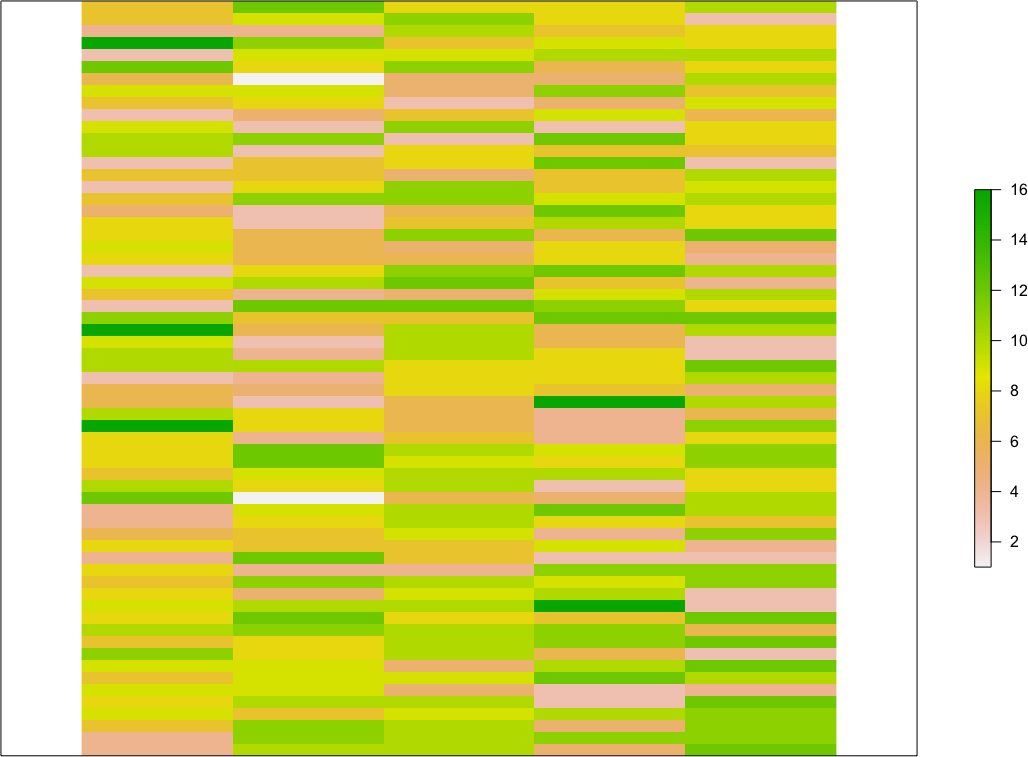
\includegraphics[width=0.8\textwidth]{fig01}
\caption{Original sequences of five virtual reels}
\label{fig:01}
\end{figure}

The fitness value estimation is done from the list of chunks, but crossover and mutation are done over candidate sequences. Such a change in the candidate sequences leads to an immediate recalculation of chunks samples. Modified uniform crossover is used with the application of normal distribution (mean 50\% and a standard deviation of 20\%) for the rate of participation of the two parents. It means that one of the parents has more influence in forming the offspring. Because the length of the original sequence is generally unknown the size of the offspring sequence length should be estimated during crossover process. As a lower bound of candidate sequence length, the number of unique symbols in the virtual reels is taken. As an upper bound of candidate sequence length, the total length of all chunks taken together is taken. Such estimation of the candidate sequence length gives chance all symbols to participate (lower bound) and all chunks to be used in a single sequence (upper bound). Such an estimation of the length gives chance to the genetic algorithm to optimize this parameter too. Almost in all cases, parents are at different lengths. The offspring differs in length from parents too. When the offspring is longer than the parents, values are taken in a loop from the beginning. It is the natural way to produce longer offspring because virtual reels are used in looping during real-time game operation. The mutation is done by random replacement of a single value in the candidate sequence. The random value is taken from the chunks of the original sequence. 

\begin{figure}[h!]
\centering
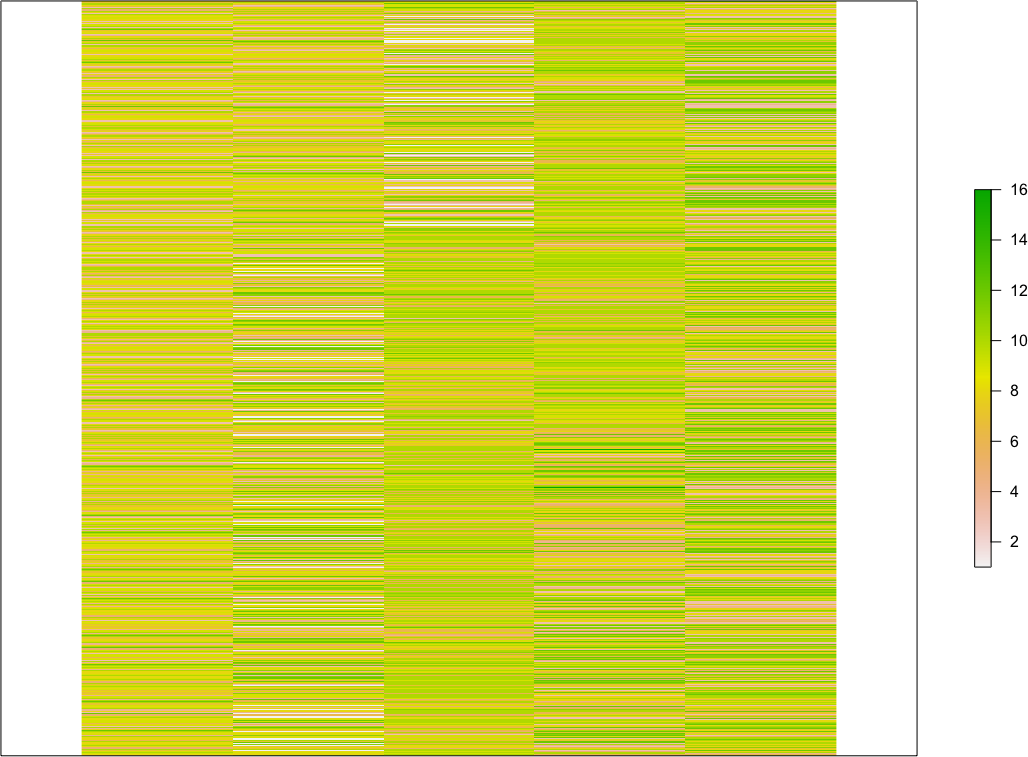
\includegraphics[width=0.8\textwidth]{fig02}
\caption{Reconstructed sequences of five virtual reels}
\label{fig:02}
\end{figure}

For the selection, three different chromosomes are selected randomly. Two of the three with better fitness are selected for parents. The third one is selected to be removed from the population and the newly generated offspring to take its place. This replacement is done only if the new offspring is better than the old one. With such a selection operator, the elitism rule is indirectly applied.

\section{Experiments and Results}

All experiments are done with a custom-created software project published in GitHub \cite{Balabanov-2020}. The source code is written in Java 8 as programming language. An empirical population of 137 individuals is chosen. The mutation rate is chosen to be 0.05\% as a recommended value in the literature. Modified competitive selection is implemented where the crossover rate is almost 100\%. Uniform crossover with a normally distributed participation threshold is chosen (mean of 50\% and standard deviation of 20\%). If the offspring is better than the worst of three individuals it takes its place and elitism rule is applied indirectly. 

A set of 8 different virtual reels is used as input data of original sequences. Visual representation of one of them is presented in Fig. \ref{fig:01}. Each of the five virtual reels is reconstructed separately. The result of the reconstructed reels is shown in Fig. \ref{fig:02}. The genetic algorithm is stated for 100 generations. It is clearly visible that reconstructed sequences are pretty different in length than the original once. Fitness values for the five reconstructed reels are as follows: -3.521716216163723, -4.310895779885775, -2.3809034389618526, -3.8553857718048152, -3.6797186696978517.

In current experiments, only a single run of genetic algorithm is done, but many consecutive runs (simulated annealing as an analogy) will improve the achieved optimality because genetic algorithms can be stuck in local optimums.

\section{Conclusion}

The presented research is an approximate sequencing of slot machine gambling games virtual reels with genetic algorithms. The optimization process in reconstruction has as criteria of optimality the distance between the observed chunks from the candidate solution and the observed chunks from the original virtual reels. Results from the experiments clearly show that the proposed approach for approximate reconstruction can be efficiently used in the industrial production of slot machine gambling games. The main application is reverse engineering of the virtual reels. Such reverse engineering could be very useful in quality control and operational control of the games. 

As for directions of further work, it will be an interesting discrete differential evolution to be used instead of genetic algorithms. In fitness estimation, Euclidean distance could be replaced with some other distance which can enforce faster optimization convergence. High-dimensional combinatorial optimization problems are usually time-consuming. In such situations, supercomputer systems as AVITOHOL \cite{Tashev-Tasheva-Petrov-2019} can be involved. A parallel implementation of population-based meta-heuristics is possible because of heir well known high degree of possible parallelism.

\section*{Acknowledgments}

This research is funded by Velbazhd Software LLC and it is partially supported by the Bulgarian Ministry of Education and Science (contract D01–205/23.11.2018) under the National Scientific Program ``Information and Communication Technologies for a Single Digital Market in Science, Education and Security (ICTinSES)'', approved by DCM \# 577/17.08.2018.

\begin{thebibliography}{99}

\bibitem{Angelova-2009} Angelova, V.: Investigations in the Area of Soft Computing Targeted State of the Art Report, Cybernetics and Information Technologies, vol. 9, no. 1, 18-24, (2009).

\bibitem{Dineva-Atanasova-2019} Dineva, K., Atanasova, T.: Methodology for Data Processing in Modular IoT System, Distributed Computer and Communication Networks, Proceedings of 22-st International Conference, Springer Nature Switzerland, vol. 11965, 457-468, (2019).

\bibitem{Borissova-Mustakerov-2015} Borissova, D., Mustakerov, I.: Open job shop scheduling via enumerative combinatorics, International Journal of Mathematical Models and Methods in Applied Sciences, vol. 9, 120-127, (2015).

\bibitem{Vaidyanathan-Phoong-1995} Vaidyanathan, P.P., Phoong, S.M.: Reconstruction of Sequences from Nonuniform Samples, Proceedings of International Symposium on Circuits and Systems, vol. 1, 601-604, (1995).

\bibitem{Lewis-1998} Lewis, P.O.: A Genetic Algorithm for Maximum-Likelihood Phylogeny Inference Using Nucleotide Sequence Data, Molecular Biology and Evolution, vol. 15, no. 3, 277-283, (1998).

\bibitem{Parsons-Johnson-1997} Parsons, R., Johnson, M.: A Case Study in Experimental Design Applied to Genetic Algorithms with Applications to DNA Sequence Assembly, American Journal of Mathematical and Management Sciences, vol. 17, no. 3-4, 369-396, (1997).

\bibitem{Tomov-Zankinski-Balabanov-2017-1} Tomov, P., Zankinski, I., Balabanov, T.: Slot Machine Reels Reconstruction with Monte-Carlo Search, Proceedings of International Scientific Conference UniTech, vol. 2, 384-387, (2017).

\bibitem{Balabanov-Ivanov-Ketipov-2020} Balabanov, T, Ivanov, S. Ketipov, R.: Solving Combinatorial Puzzles with Parallel Evolutionary Algorithms, Proceedings of International Conference on Large-Scale Scientific Computing, Lecture Notes in Computer Science, vol. 11958, 493-500, (2020).

\bibitem{Tomov-Zankinski-Balabanov-2019} Tomov, P., Zankinski, I., Balabanov, T.: Genetic Algorithm Selection Operator Based on Recursion and Brute-Force, Abstracts of Annual Meeting of the Bulgarian Section of SIAM, Fastumprint, 93-93, (2019).

\bibitem{Balabanov-Sevova-Kolev-2019} Balabanov, T., Sevova, J, Kolev, K.: Optimization of String Rewriting Operations for 3D Fractal Generation with Genetic Algorithms, Proceedings of International Conference on Numerical Methods and Applications, Lecture Notes in Computer Science, vol. 11189, 48-54, (2019).

\bibitem{Balabanov-Barova-Keremedchiev-2016} Balabanov, T, Barova, M., Keremedchiev, D.: Image Construction with 2D Ellipses by Genetic Algorithms Optimization, Abstracts of Annual Meeting of the Bulgarian Section of SIAM, Fastumprint, 10-11, (2016).

\bibitem{Balabanov-Zankinski-Barova-2016} Balabanov, T, Zankinski, I., Barova, M.: Strategy for Individuals Distribution by Incident Nodes Participation in Star Topology of Distributed Evolutionary Algorithms, Cybernetics and Information Technologies, vol. 16, no. 1, 80-88, (2016).

\bibitem{Balabanov-Zankinski-Dobrinkova-2011} Balabanov, T, Zankinski, I., Dobrinkova, N.: Time Series Prediction by Artificial Neural Networks and Differential Evolution in Distributed Environment, Proceedings of International Conference on Large-Scale Scientific Computing, Lecture Notes in Computer Science, vol. 7116, 198-205, (2011).

\bibitem{Balabanov-Zankinski-Shumanov-2015} Balabanov, T, Zankinski, I., Shumanov, B.: Slot Machine RTP Optimization and Symbols Wins Equalization with Discrete Differential Evolution, Proceedings of International Conference on Large-Scale Scientific Computing, Lecture Notes in Computer Science, vol. 9374, 210-217, (2015).

\bibitem{Tomov-Zankinski-Balabanov-2017-2} Tomov, P., Zankinski, I., Balabanov, T: Slot Machine Reels Reconstruction with Genetic Algorithms, Abstracts of Annual Meeting of the Bulgarian Section of SIAM, Fastumprint, 102-103, (2017).

\bibitem{Balabanov-2020} Balabanov, T.: Approximated Sequences Reconstruction with Genetic Algorithms, https://github.com/TodorBalabanov/Approximated-Sequences-Reconstruction-with-Genetic-Algorithms

\bibitem{Tashev-Tasheva-Petrov-2019} Tashev, T., Tasheva, R., Petrov, P.: Determination of the Computer Modelling Precision for Throughput of Switch Node with LPF-algorithm, Proceedings of  International Conference on Computer Systems and Technologies, ACM, 141-145, (2019).

\end{thebibliography}

\end{document}
